\section{Field Study} % (fold)
\label{sec:field_study}

In the end of the project we tested the visualization directly in school in two different sessions with respect to the two different target groups: In one class the teacher used \HG as a teaching material and in another class the students used it as a study material to research about an historical topic.

\subsection{Teaching Material} % (fold)
\label{sub:usage_as_teaching_material}

Our research question for the first test was if \HG is suitable as a teaching material in the classroom. The teacher wanted to use the software to explain the historical context (name, time and location), the content and the consequences of four major conferences at the end of World War II: Casablanca and Tehran 1943, Yalta and Potsdam 1945.

\subsubsection{Planning} % (fold)
\label{ssub:planning-1}

% We had the following research hypotheses:
% \begin{enumerate}
%   \item Effectiveness $H_{efs-1.1}$: \HG is well suited to impart the historical context (What?, When?, Where?, How?) of an historical event.
%   \item Effectiveness $H_{efs-1.2}$: \HG is not suited to impart the historical coherences (Why?) of historical events.
%   \item Satisfaction $H_{sat-1.1}$:  The teacher will have no technical oder usability problem while presenting the topic with \textsc{HistoGlobe}.
%   \item Satisfaction $H_{sat-1.2}$:  The students will appreciate the visualization of the topic with \textsc{HistoGlobe}.
% \end{enumerate}

Because there is just one test in one class with one teacher and the course of a history class is somewhat arbitrary, we did not use any quantitative measures to answer our research question. Our main focus was finding out whether the current concept of \HG is suited as a teaching material and if there are major usability flaws. We decided to use the following methods:

\begin{enumerate}
  \item Video recording of the whole class to analyze the usage of the teacher afterwards.
  \item Semi-structural interview with the teacher after the class to get more insight into his usage of the software.
  \item Short Questionnaire (see: appendix \ref{ssub:questionnaires}) for the students after the class.
\end{enumerate}

% subsubsection planning (end)

\subsection{Conduction} % (fold)
\label{sub:conduction-1}
On Thursday, 16.04.2015 from 11:35 until 13:05 the teacher held a lesson about the four major conferences after World War II. In 15 minutes during the lesson he actively used \HG to show the students the location, the date, the name and an image of the conference. He asked the students about the context and content of the conferences using the visualization. He swapped between his own prepared teaching slides and \HG. He once used the software spontaneously (see Figure \ref{fig:teacher}): A student asked ``What is a satellite state?'', and the teacher explained it by the Soviet satellite sates (GDR, Poland, Czechoslovakia and alike).

\begin{figure}[ht]
  \begin{center}
    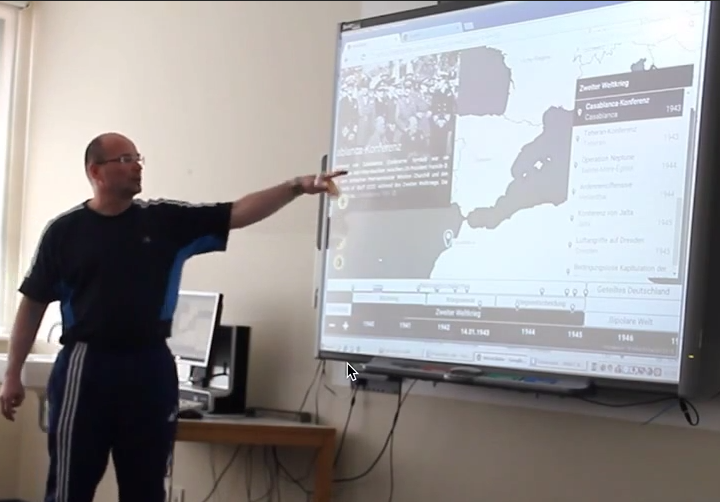
\includegraphics[width=0.4\textwidth]{graphics/teacher-2.png}
    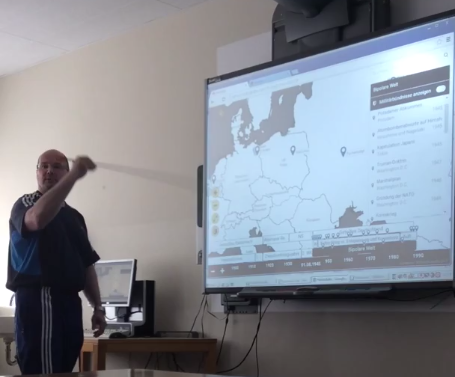
\includegraphics[width=0.4\textwidth]{graphics/teacher-1.png}
  \end{center}
  \caption{The usage of \HG as a teaching material in the classroom}
  \label{fig:teacher}
\end{figure}

% subsection conduction (end)

\subsection{Results} % (fold)
\label{sub:results-1}

While the teacher used \HG we noticed the following:

\begin{itemize}
  \item The Hivent List was the only element he used to select an Hivent, neither the Timeline nor the Map.
  \item The visualization was only in the high contrast mode. It seemed suitable for the very bright lighting condition.
  \item The teacher used only the mouse, not the Smartboard, as an input device.
  \item Sometimes there are labels of minor countries on the map, but the important ones are missing. The label display concept has to be thought through again.
  \item The current date of the visualization is barely visible and should be more prominent.
\end{itemize}

In the interview with the teacher after the lesson we revealed the following important results of the field study:

\begin{itemize}
  \item The big advantage of \HG is the map, especially navigation and zooming.
  \item The teacher sees great potential in visualizing territorial development of countries and membership to alliances.
  \item \HG is suited for him to show the name, date and location of an Hivent, but not the coherences. In his opinion this shall also not be the focus of the software.
  \item He believes that the effect on the students is only minor, because they are used to work with a Smartboard and \HG does not give them extra information
\end{itemize}

The students gave us valuable feedback in the questionnaire (Figure \ref{fig:studyresults-1}):

\begin{itemize}
  \item Most students found \HG interesting, became curious about the software and are willing to work more with \HG
  \item The biggest advantages seem to be the summary and the overview that the visualization gives to them. Also the factor of time and the picturing of the Hivents because of the images seem well-made.
  \item Most students did not appreciate the black-and-white design of the HighContrast mode and were confused by the visualization.
  \item Some students complained that \HG was not used enough in class in order to understand and appreciate it more.
\end{itemize}

\begin{figure}[H]
  \begin{center}
    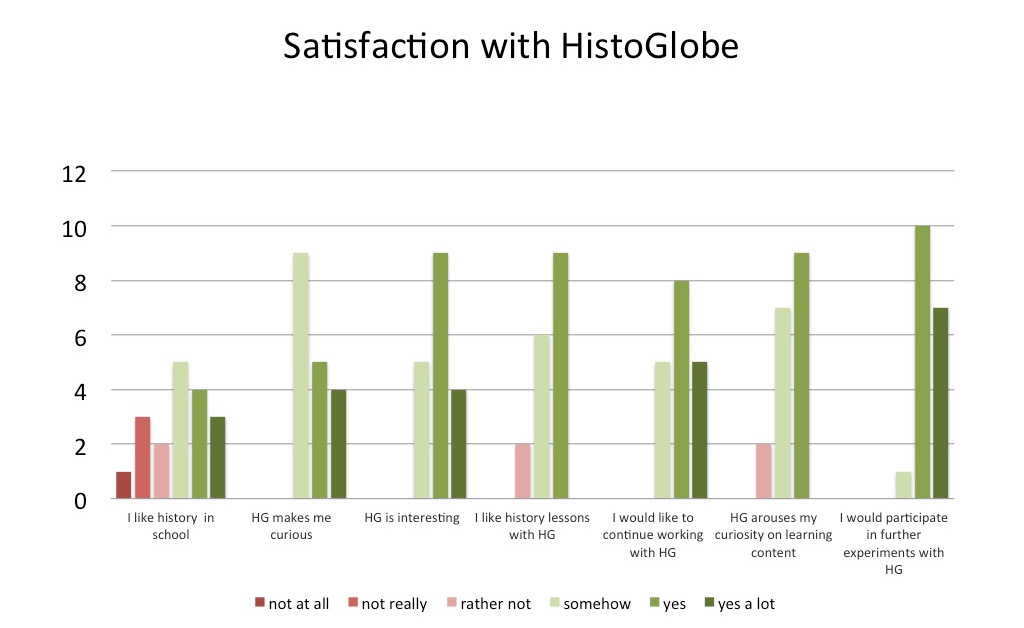
\includegraphics[width=0.9\textwidth]{graphics/test-1-satisfaction.jpg} \\[0.5em]
    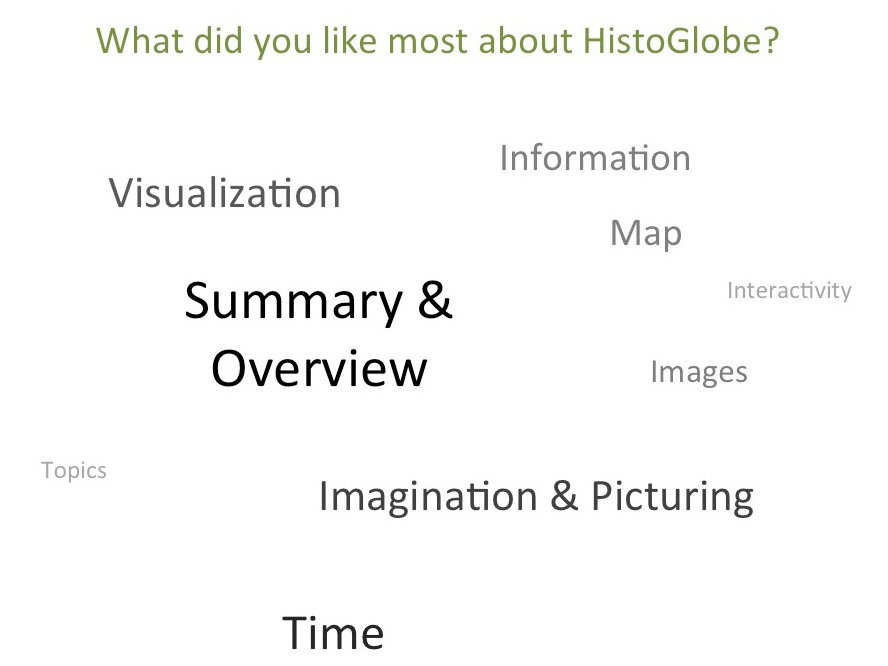
\includegraphics[width=0.45\textwidth]{graphics/test-1-tagcloud-pos.jpg}
    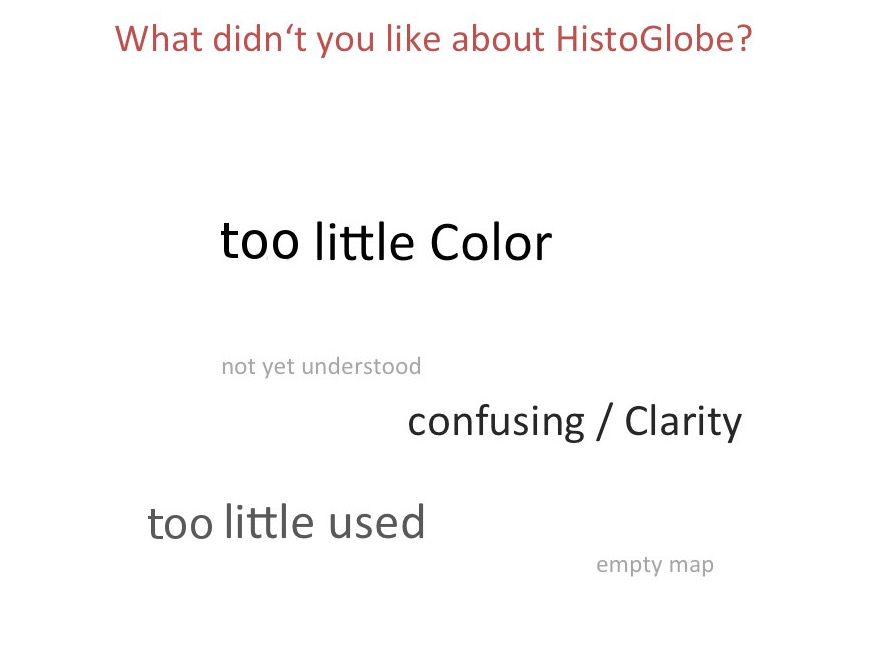
\includegraphics[width=0.45\textwidth]{graphics/test-1-tagcloud-neg.jpg}
  \end{center}
  \caption{Results of the first field study with students}
  \label{fig:studyresults-1}
\end{figure}

We conclude from the feedback of the teacher and the students that \HG is only partially useful as a teaching material -- but we believe it was much more helpful for students to learn.

% Finally, we see potential evidence for accepting our research hypotheses. It seems to be that \HG is well suited to impart the \textit{What?, When?, Where?} and \textit{How?} of an Hivent ($H_{efs-1.1}$) but not at all for the explanation of the \textit{Why?}: historical coherences ($H_{efs-1.2}$). From our observation, hypothesis $H_{sat-1.1}$ seems to hold and also $H_{sat-1.1}$ is also likely due to the results from the questionnaire. It has to mentioned that this analysis is neither exhaustive nor statistically accurate, because we have not conducted a classical user study.

% subsection results (end)
% subsection usage_as_teaching_material (end)


\subsection{Study Material} % (fold)
\label{sub:usage_as_study_material}

One week later we had the chance to examine this research question: \HG is suitable as a study material to research about historical topics. In a computer pool of Lobdeburgschule the students workes on the task to inform themselves about events in the cold and the hot phases of the Bipolar World 1945-1993. The output was supposed to be a timeline with an overview about the development in the Bipolar World.

% We had the following research hypotheses:
% \begin{enumerate}
%   \item Effectiveness $H_{efs-2.1}$: \HG is well suited to understand the historical context (What?, When?, Where?, How?) of an historical event.
%   \item Effectiveness $H_{efs-2.2}$: \HG is not suited to understand the historical coherences (Why?) of historical events.
%   \item Satisfaction $H_{sat-2.1}$: The students will have no technical oder usability problems while doing research with \textsc{HistoGlobe}.
% \end{enumerate}

\subsubsection{Conduction} % (fold)
\label{ssub:conduction-2}
On Friday, 22.04.2015, from 11:35 until 13:05 the students performed the task stated above. We used the time to find out about the usage of \HG and the advantages, disadvantages and problems with the software.

In the same way as in the first field study we only used qualitative methods to evaluate our hypotheses. We observed the students while working, asked specific questions and used the same questionnaire as the week before to measure a difference between the usage of \HG for teaching and for learning purposes.

\begin{figure}[tb]
  \begin{center}
    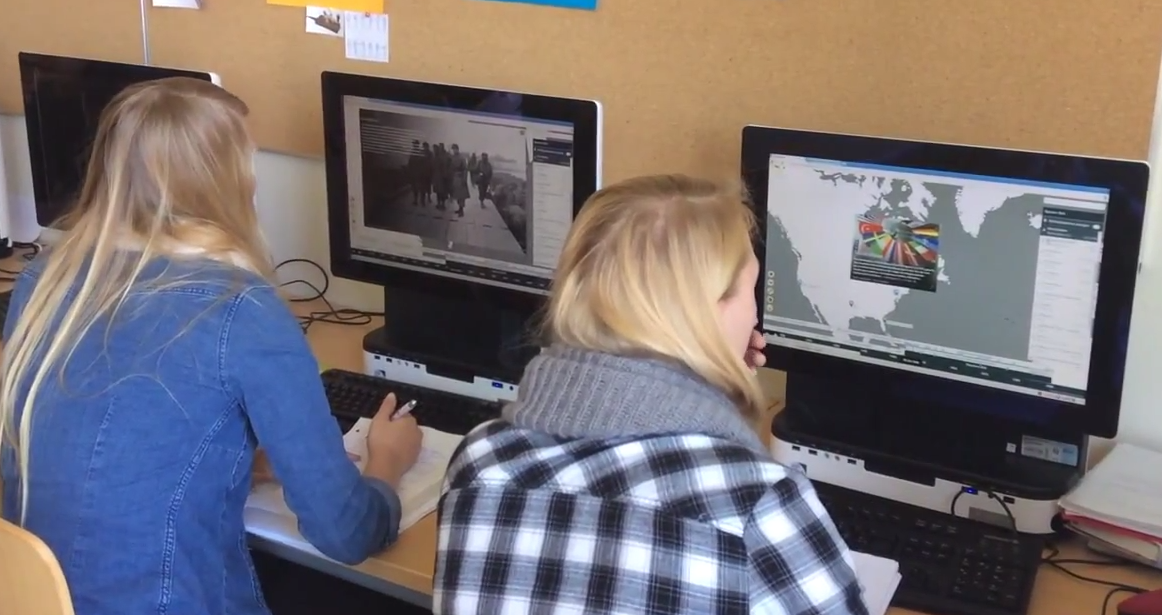
\includegraphics[width=0.45\textwidth]{graphics/students-1.png}
    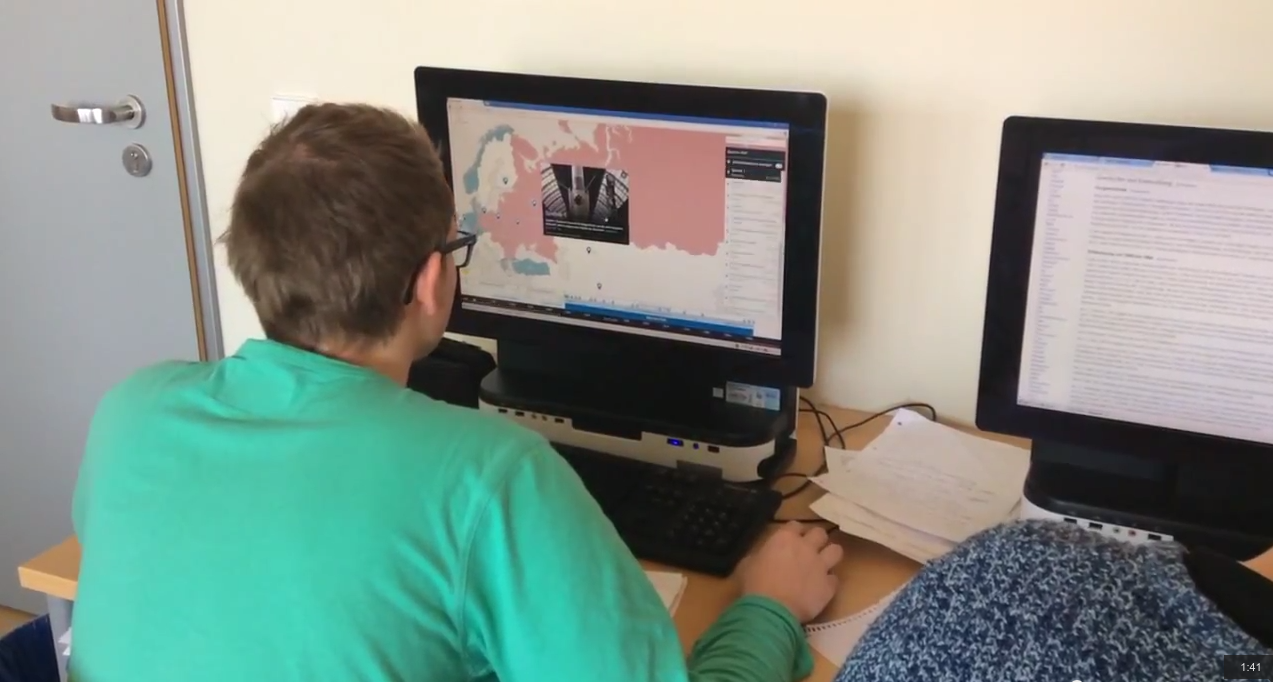
\includegraphics[width=0.45\textwidth]{graphics/students-2.png}
    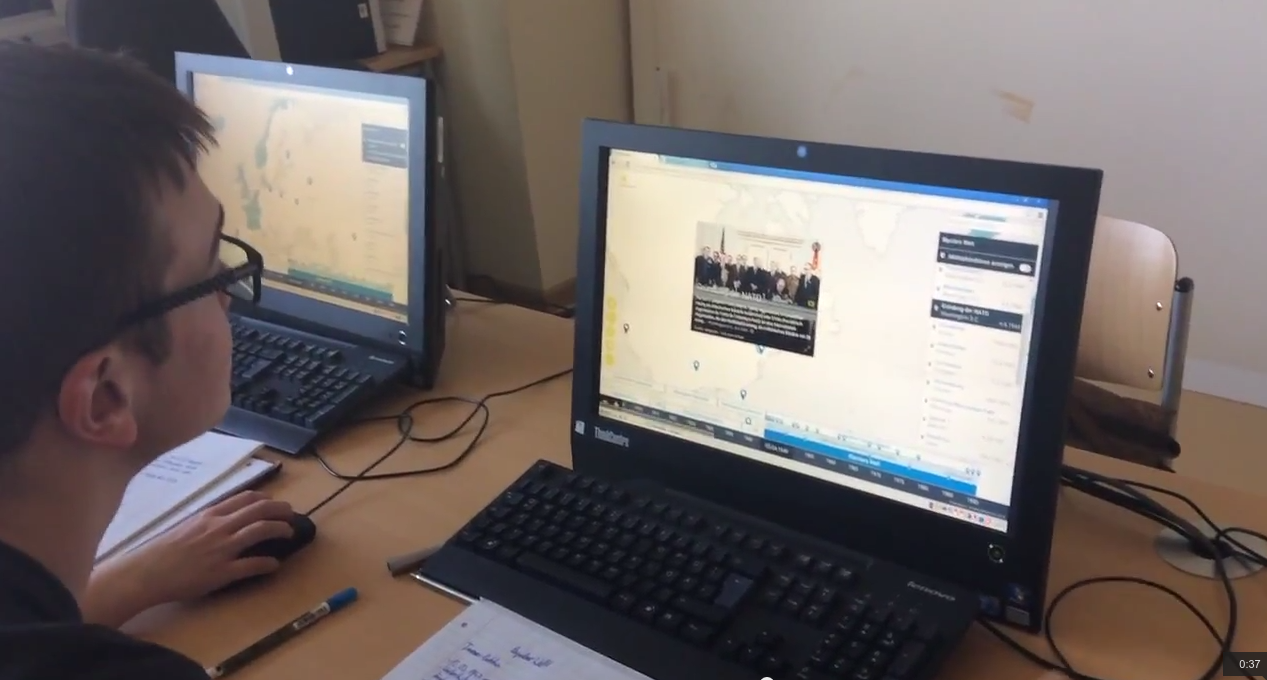
\includegraphics[width=0.45\textwidth]{graphics/students-3.png}
    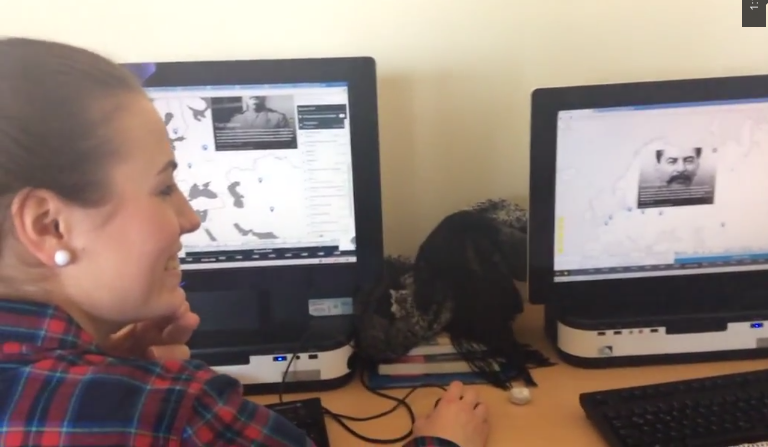
\includegraphics[width=0.45\textwidth]{graphics/students-4.png}
  \end{center}
  \caption{The usage of \HG as a learning material for the students}
  \label{fig:students}
\end{figure}

% subsubsection conduction (end)

\subsubsection{Results} % (fold)
\label{ssub:results-2}

While observing the students working we registered several interesting things:
\begin{itemize}
  \item There were no questions from the students how to use the software, everyone was able to use it form the beginning.
  \item The software was worked smoothly on the machines.
  \item The students clicked on the topic ``Bipolar World'' and clicked on each Hivent in the Hivent List one after the other. They opend the Hivent Box in full screen and read the short article. They did use neither the Timeline nor the Map actively.
  \item Some students used the Wikipedia link to get to know more about an Hivent. Only one student has searched on Google fr additional information.
  \item One problem for the students was to find out which Hivents are important, because all seem equally relevant.
\end{itemize}

We collected feedback to each User Interface element during the observation and in a feedback session after the class:
\begin{itemize}
  \item The Map was almost exclusively used passively. The information on the Map was widely understood, especially the alliances were considered as helpful. Since there were no major border changes between 1945 and 1992, we could did find out if the visualization of border changes were helpful. One requested feature was cities on the map for a better orientation.
  \item The Timeline was not used, except by some students for the development of the bipolar alliances. Also the topics bar was only used once for selecting Bipolar World. The Hivent markers on the Timeline were not helpful, because there was no visible connection between name of the HIvent and the marker.
  \item The Hivent List was the main navigation element, the only one that was actively used by all students the whole time. It was considered to be very helpful to know which event happened where and when.
  \item The Search Bar was not used at all by anybody. This is probably because of the exploratory nature of the task from the teacher.
  \item The Hivent Boxes were the main source of information. Everybody liked the content and the style of the box, especially the image of the Hivent. The box is very powerful, because most students directly copied the content from the box in their notes.
  \item Half of the students used the high contrast mode even if it was not necessary with respect to the lighting conditions. It seems like it is visually appealing. For the other control buttons we did not observe anything special.
\end{itemize}

\begin{figure}[H]
  \begin{center}
    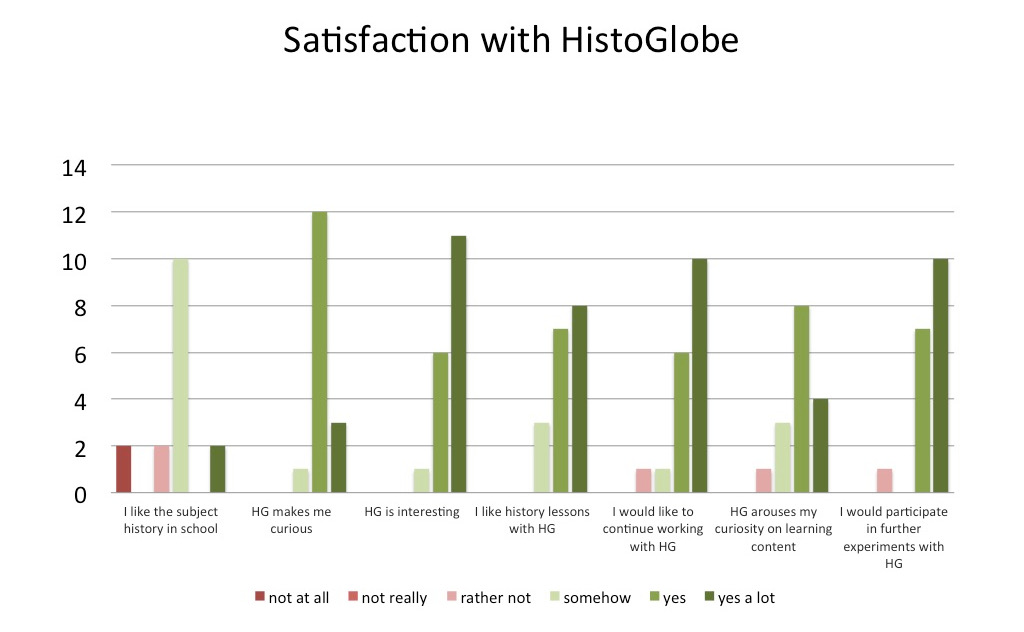
\includegraphics[width=0.9\textwidth]{graphics/test-2-satisfaction.jpg} \\[0.5em]
    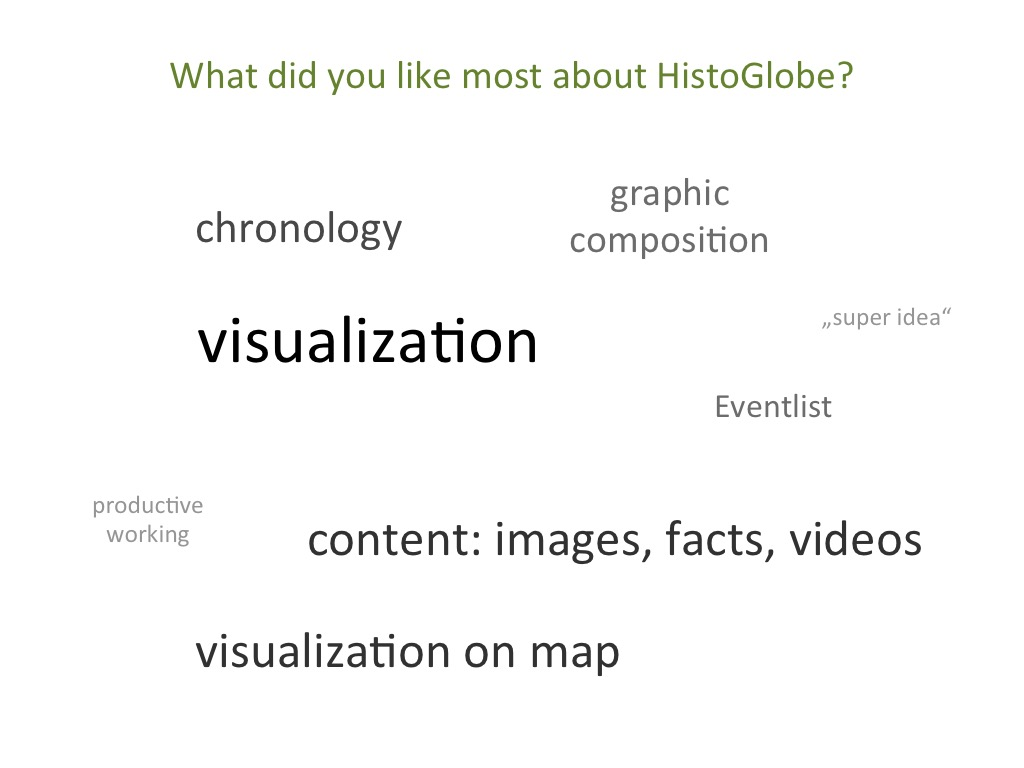
\includegraphics[width=0.45\textwidth]{graphics/test-2-tagcloud-pos.jpg}
    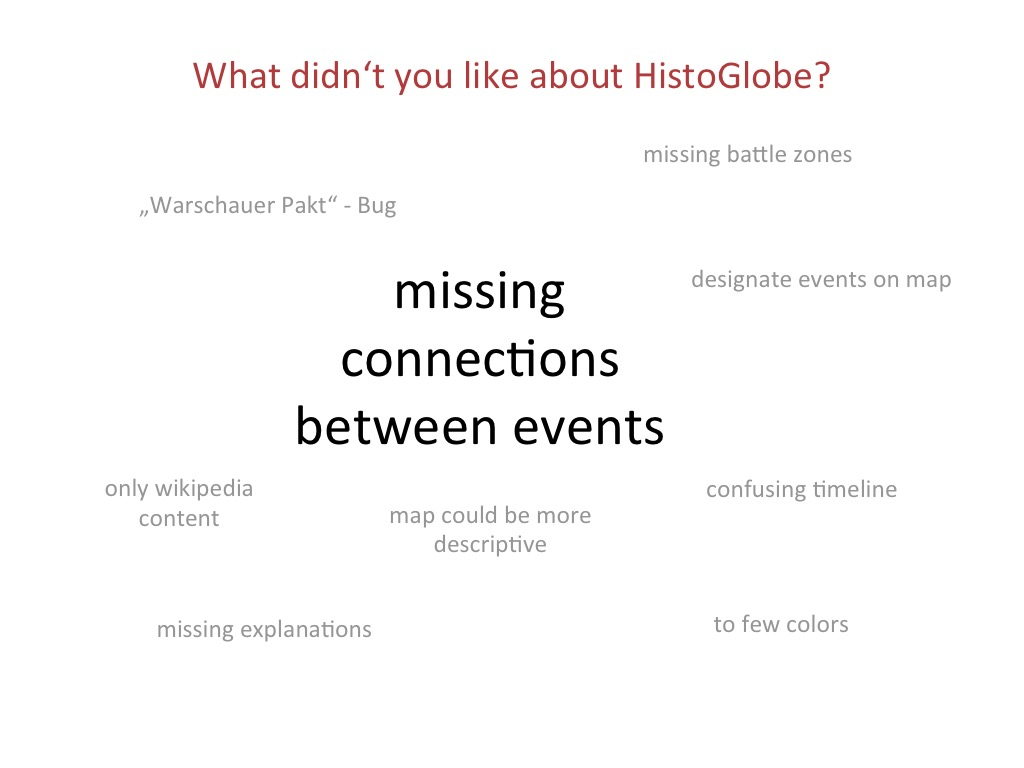
\includegraphics[width=0.45\textwidth]{graphics/test-2-tagcloud-neg.jpg}
  \end{center}
  \caption{Results of the second field study with students}
  \label{fig:studyresults-2}
\end{figure}

From the results of the questionnaire (figure \ref{fig:studyresults-2}) it becomes clear that especially the vividness of the visualization, the chronology and the visual impressions of the Hivents were very helpful. While there were smaller problems and feature requests mentioned by particular students, one big problem arose by most: \HG does not answer the \textit{Why}-question: There are no coherences visible.

% Finally we can see some potential evidence for accepting our research hypotheses: Regarding $H_{efs-2.1}$ and $H_{efs-2.2}$: \HG was said by most students to be helpful for understanding the historical context (What?, When?, Where?, How?) but not the historical coherences (Why?) of historical events. The third hypothesis $H_{sat-2.1}$ has also a high probability of being valid, since no student asked a question regarding the usability of the system, moreover they appreciated it a lot.

Overall, most students were satisfied with \HG, because it is easy and fun to use, has a plausible usability and gives a good overview about what happened. Even the teacher said in the end, that for the task he has given the students \HG is very suitable -- because it is good for getting an overview, but not for detailed discussions about history.

% subsubsection results (end)
% subsection usage_as_study_material (end)
% section field_study (end)
